\section{Beschreibung}
In dieser Übung wird eine \emph{DSL} entwickelt, mit der ein Modul für eine bestehende Anwendung beschrieben werden kann. Mit dieser Beschreibung wird eine Maven-Projektstruktur sowie Java Quelltexte wie folgt aufgelistet erstellt:
\begin{itemize}
	\item\emph{\textbf{[module\_key]}/message/pom.xml}
	\newline
	Das Projekt der \emph{Message Bundles}.

\begin{itemize}
	\item\emph{/message/../com.clevercure.\textbf{[module\_key]}.message.\textbf{[bundle\_name]}MessageBundle.java}
	\newline
	Der Aufzählungsdatentyp mit den Schlüsseln der sprachspezifischen Texte.

	\item\emph{/message/../resources/META-INF/resource-bundles/\textbf{[bundle\_name]\_[locale]}.properties}
	\newline
	Die \emph{Locale}-spezifische \emph{Properties}-Datei mit den sprachspezifischen Texten.	
	\end{itemize}
	
	\item\emph{\textbf{[module\_key]}/model/pom.xml}
	\newline
	\emph{Parent} für alle Modell Projekte.
	
	\item\emph{\textbf{[module\_key]}/model/jpa/pom.xml}
	\newline
	Das Projekt der \emph{JPA}-Modells.
	\begin{itemize}
		\item\emph{/jpa/../com.clevercure.\textbf{[module\_key]}.jpa.observer.Observer.java}
		\newline
		Die \emph{Observer}-Klasse, die auf die definierten \emph{Events} reagiert.	
		\item\emph{/jpa/../resources/META-INF/\textbf{[module\_key]}Orm.xml}
		\newline
		Die \emph{JPA 2.2 orm.xml} Konfigurationsdatei.	
		\item\emph{/jpa/../resources/META-INF/beans.xml}
		\newline
		Die \emph{CDI 1.1} Konfigurationsdatei, die \emph{CDI} für dieses Artefakt aktiviert.	
	\end{itemize}
	
	\item\emph{\textbf{[module\_key]}/service/pom.xml}
	\newline
	\emph{Parent} für alle Service Projekte.
	
	\item\emph{\textbf{[module\_key]}/service/api/pom.xml}
	\newline
	Das Projekt mit der Service Spezifikation

	\item\emph{\textbf{[module\_key]}/service/impl/pom.xml}
	\newline
	Das Projekt mit der Service Implementierung.
	\begin{itemize}
		\item\emph{/service/impl/../com.clevercure.\textbf{[module\_key]}.service.impl.observer.Observer.java}
		\newline
		Die \emph{Observer}-Klasse, die auf die definierten \emph{Events} reagiert.
		\item\emph{/service/impl/../resources/META-INF/beans.xml}
		\newline
		Die \emph{CDI 1.1} Konfigurationsdatei, die \emph{CDI} für dieses Artefakt aktiviert.	
	\end{itemize}
\end{itemize}
\ \newline
Es können folgende Aspekte eines Moduls beschrieben werden:
\begin{itemize}
	\item\textbf{\emph{MessageBundles}} sind Beschreibungen von Klassen, die sprachspezifische Texte für einen Schlüssel und eine \emph{Locale} verwalten.
	
	\item\textbf{\emph{Observers}} sind Beschreibungen von Beobachtermethoden, die mittels einen \emph{Delegate} auf einem definierten \emph{CDI}-Event reagieren können.
	
	\item\textbf{\emph{JpaConfig}} ist die Beschreibung des \emph{JPA}-Projekts, dem \emph{Observer} und \emph{MessageBundles} hinzugefügt werden können.
	
	\item\textbf{\emph{ServiceConfig}} ist die Beschreibung der \emph{Service}-Projekte, dem \emph{Observer} und \emph{MessageBundles} hinzugefügt werden können.
\end{itemize}
\ \newline
Das Ziel dieser \emph{DSL} ist es den initialen Aufwand beim Erstellen eines Moduls für eine bestehende Anwendung zu erleichtern. Ein Module besteht aus mehreren \emph{Maven}-Projekten und Konfigurationsdateien, die Mühsam erstellt werden müssen. Mit dieser \emph{DSL} kann ein Modul einfach beschrieben werden und daraus einen \emph{Maven}-Projektstruktur, mit Konfigurationsdateien und Java Quelltexten zu erstellen.
\begin{figure}[h]
	\centering
	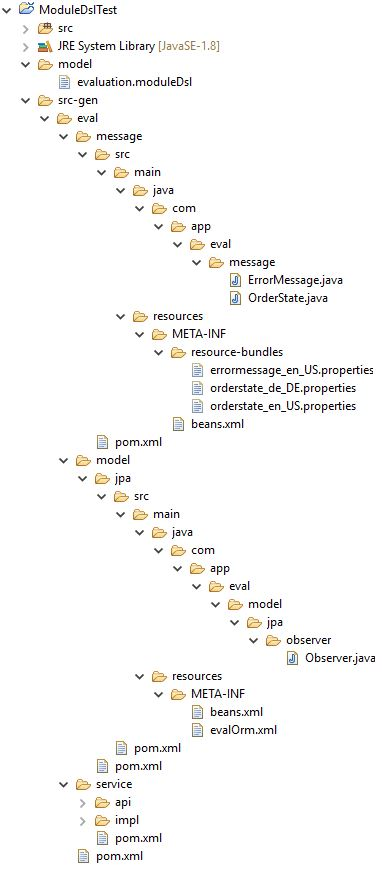
\includegraphics[scale=0.8]{\imageDir/test_project_with_generated.JPG}
	\caption{Testprojekt für das Modul mit generierten Ressourcen}
	\label{fig:3-test}
\end{figure}
\ \newpage

